\documentclass{beamer}
%\documentclass[handout,numbers]{beamer}
%\documentclass[handout,draft]{beamer}
%\includeonlyframes{current}
\usepackage{pgfpages}
\usepackage[english]{babel}
%\usepackage[latin1]{inputenc}
%\usepackage{times}
%\usepackage[T1]{fontenc}
\usepackage{versions}
\includeversion{TOKEEPSECRET}
\excludeversion{INUTILE}
\newcommand{\OPT}{\mbox{\rm OPT}}
\newcommand{\A}{\mathcal{A}}
\newcommand{\Ss}{\mathcal{S}}

\mode<handout>{
  \setbeameroption{show notes}
  \pgfpagesuselayout{4 on 1}[letterpaper,border shrink=5mm,landscape]
  % instead of   \pgfpagelayout{4 on 1}[border shrink=5mm,landscape]
  \setbeamercolor{background canvas}{bg=black!5}
}
\mode<presentation>
{
  \usetheme{Warsaw}
  \setbeamercovered{transparent}
  \setbeamertemplate{footline}{\hfill\insertframenumber/\inserttotalframenumber} 
  \AtBeginSection[]
  {
    \begin{frame}<beamer>
      \frametitle{Outline}
      \tableofcontents[currentsection]
    \end{frame}
  }
}


\title[Instance Optimality] 
{From Fine Grained Analysis to Instance Optimality}
\author{J{\'e}r{\'e}my Barbay}

\begin{INUTILE}
\begin{abstract}
Surprisingly enough, an algorithm exists for computing 2-d or 3-d convex hulls that is optimal for every point set [FOCS 2009], in the worst case over input order: this is called "Input Order Oblivious Instance Optimality". I will describe the history and intuition behind this result, and which future similar results can be expected.
\end{abstract}
\end{INUTILE}
\institute
{
  jeremy@barbay.cl
}

\date{[2016-10-19 Wed 17:00-17:30]@Santiago}
\subject{Talks}


% If you wish to uncover everything in a step-wise fashion, uncomment
% the following command: 
%\beamerdefaultoverlayspecification{<+->}


\begin{document}

\begin{frame}
  \titlepage
\end{frame}

\begin{frame}
  \frametitle{Outline}
  \tableofcontents
  % You might wish to add the option [pausesections]
\end{frame}


\section{The Convex Hull Paradox}

\begin{frame}<presentation>
  \frametitle{The Planar Convex Hull}
  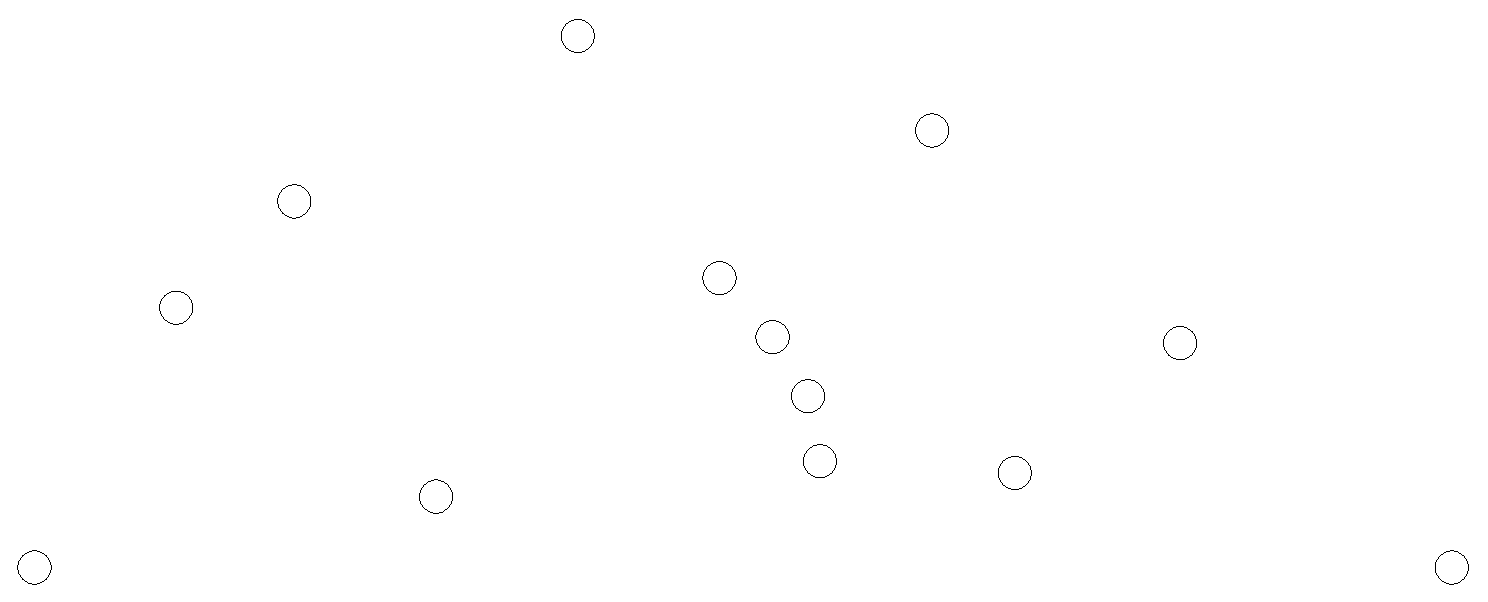
\includegraphics[width=\textwidth]{points}
  \begin{itemize}
  \item Can one of you define it?
  \item What is the best complexity known for it?
  \end{itemize}
\end{frame}


\subsection{$O(n\lg n)$}
\begin{frame}
  \frametitle{2d Convex Hull in $O(n\lg n)$}
  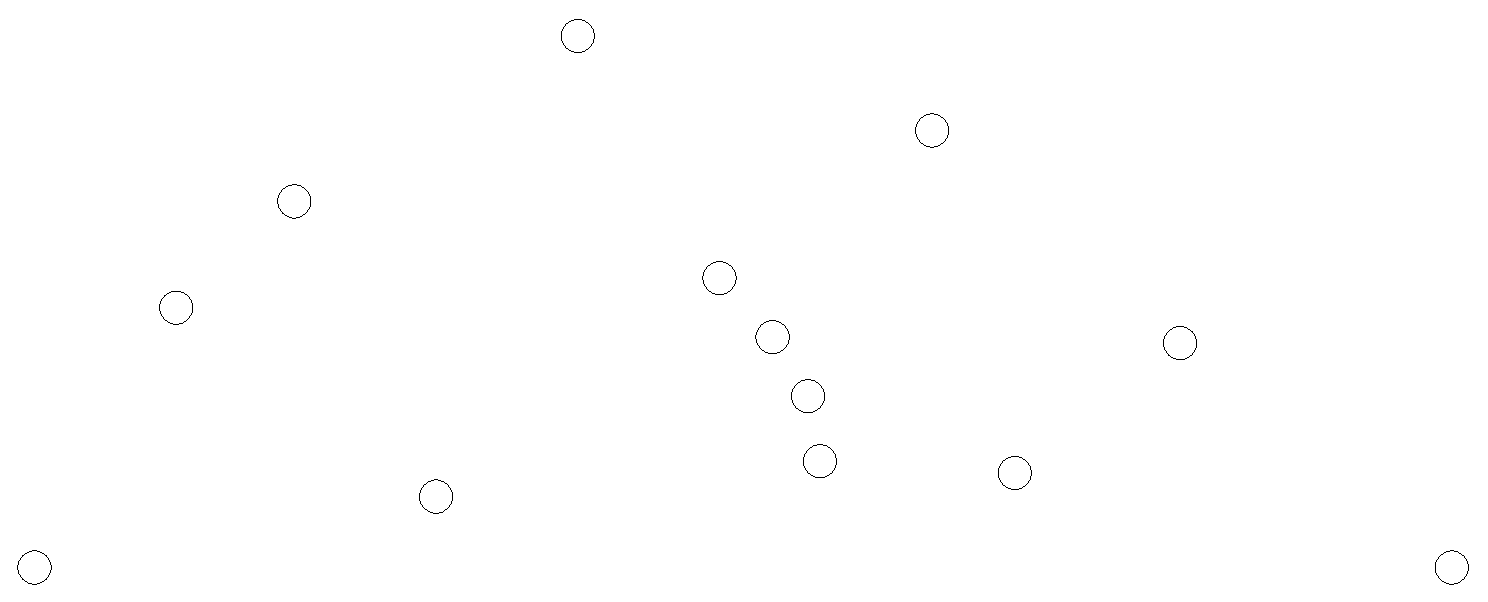
\includegraphics[width=\textwidth]{points}
  \begin{enumerate}
  \item Sort the points by $x$-coordinates;
  \item Scan them, backtracking if necessary.
  \end{enumerate}
\end{frame}



\subsection{$O(nh)$}
\begin{frame}
  \frametitle{2d Convex Hull in $O(nh)$}
  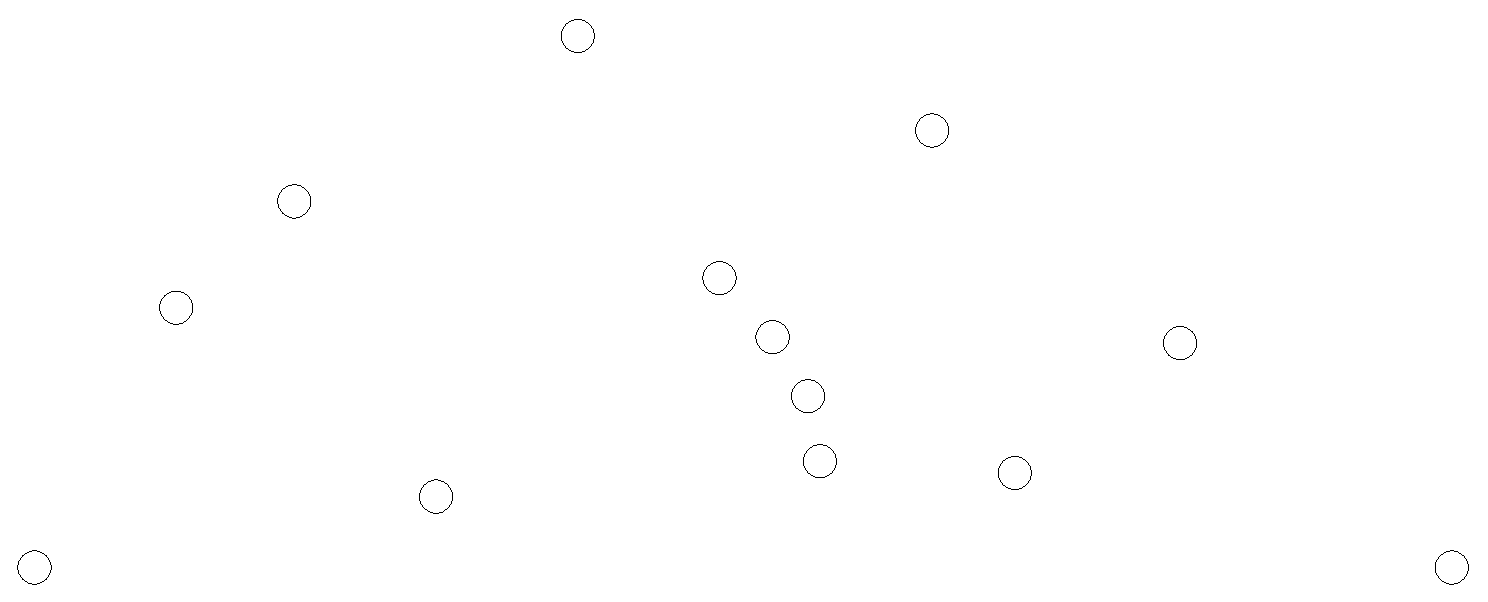
\includegraphics[width=\textwidth]{points}
  \begin{enumerate}
  \item Find the left-most point
  \item Compute the $n-1$ slopes with the other points
  \item Choose the highest slope
  \item Iterate 
  \end{enumerate}
\end{frame}


\subsection{Worst Case Complexity?}

\begin{frame}
  \frametitle{Worst case Complexity of 2d Convex Hull}
  \begin{itemize}
  \item Question ill-defined: the worst case over what?
    \begin{itemize}
    \item all instances of fixed size $n$?
    \item all instances of fixed input size $n$ and output size $h$?
    \end{itemize}
  \item For each we have distinct lower bounds:
    \begin{itemize}
    \item $\Omega(n\lg n)$, which is tight; and
    \item $\Omega(n\lg h)$, which is \alert{not} tight! \\
{\tiny (compared to the $O(nh)$ algorithm mentioned in the previous slide)}
    \end{itemize}
  \item So what is the complexity of 2d convex hull?
  \end{itemize}
\end{frame}



\section{Fine grained analysis of the convex hull}

\subsection{$O(n\lg h)$ in 2D}
\begin{frame}
  \frametitle{2d Convex Hull in $O(n\lg h)$ in 2D}
  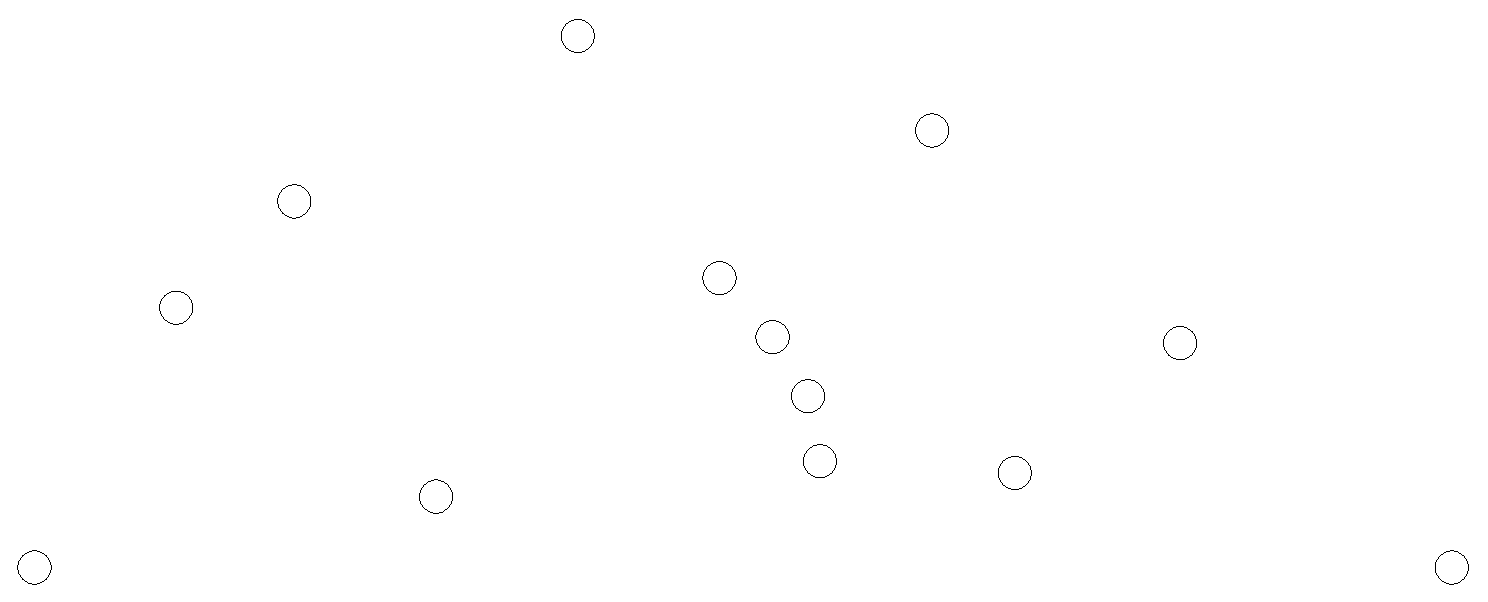
\includegraphics[width=\textwidth]{points}
  \begin{enumerate}
  \item Compute the point $m$ of median $x$-coordinate;
  \item Partition the points by $m.x$;
  \item Compute the highest edge $(a,b)$ intersecting the line $x=m.x$;
  \item Recurse on each side;
  \end{enumerate}
\end{frame}

\subsection{$O(n\lg h)$ in 3D}
\begin{frame}
  \frametitle{2d Convex Hull in $O(n\lg h)$ in 3D}
  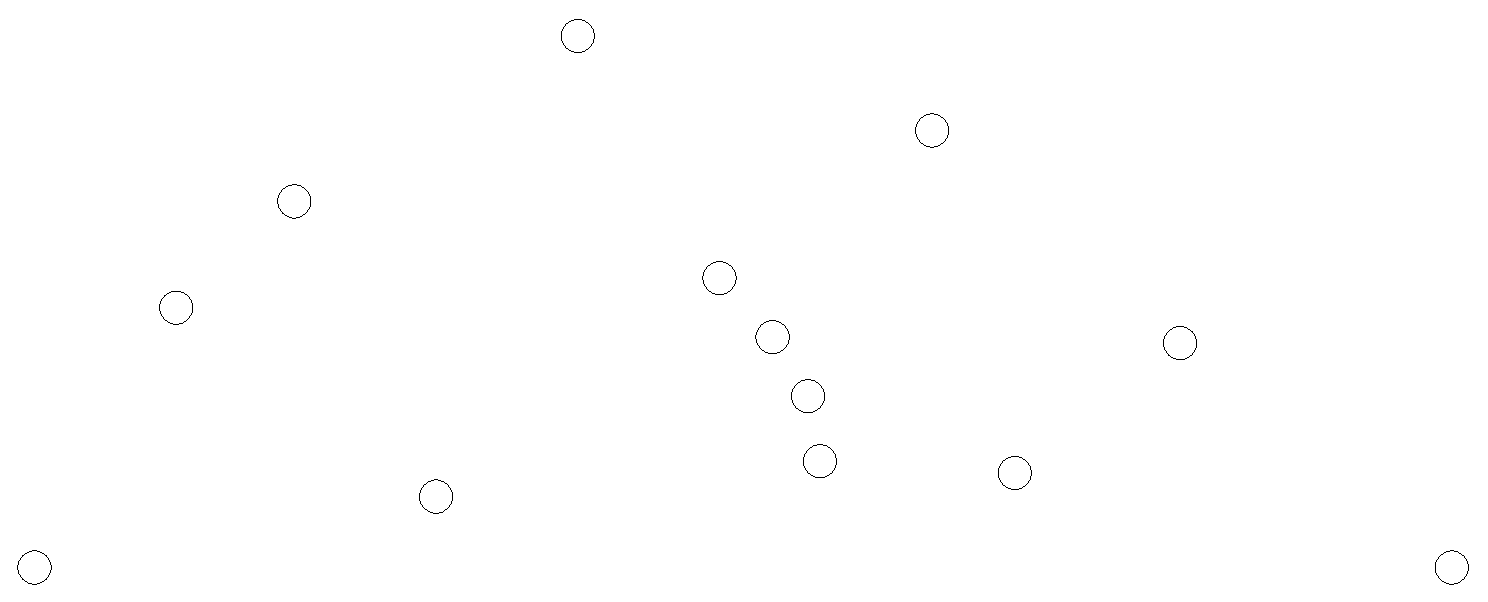
\includegraphics[width=\textwidth]{points}
  \begin{enumerate}
  \item Start with a small guess for $h$;
  \item Group the instances in $n/h$ $x$-sorted groups of size $h$;
  \item Simulate the $O(nh)$ algorithms on the groups;
  \item If it did not suffice, merge the group two by two and iterate.
  \end{enumerate}
\end{frame}

\subsection{$O(n H(C))$, instance optimal}

\begin{frame}
  \frametitle{Convex Hull in $O(n(1+H(C)))$}
  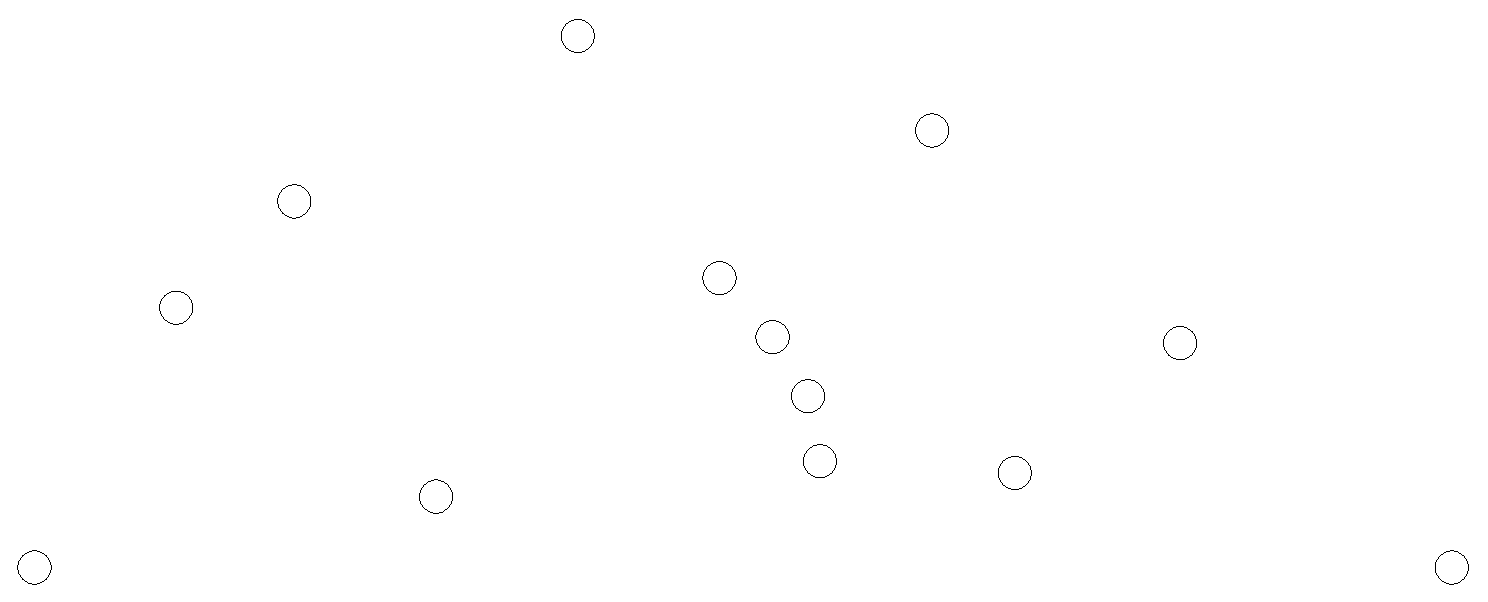
\includegraphics[width=\textwidth]{points}
  \begin{itemize}
  \item Algorithm: a variant of [Kirkpatrick, Seidel]
    \begin{enumerate}
    \item Compute the points leftmost $l$ and rightmost $r$;
    \item Compute the point $m$ of median $x$-coordinate;
    \item Compute the highest edge $(a,b)$ intersecting the line $x=m.x$;
    \item Remove all points contained in the polygon $(l,a,b,r)$;
    \item Recurse on each side;
    \end{enumerate}
  \end{itemize}
\end{frame}

\begin{frame}
  \frametitle{Instance Optimality: definitions}
  
  \begin{definition}[Instance Optimality]
    An algorithm is \alert{instance-optimal} if its cost is at most a
    constant factor from the cost of any other algorithm $A'$ running on
    the same input, for {\em every} input instance.
  \end{definition}
  
  Unfortunately, for many problems, this requirement is too stringent. 
  
  \begin{definition}[Input Order Oblivious Instance Optimality]
    For a set $S$ of $n$ elements in ${\cal D}$, let $T_A(S)$ denote
    the maximum running time of $A$ on input $\sigma$ over all $n!$
    possible permutations $\sigma$ of $S$.  Let $\OPT(S)$ denote the
    minimum of $T_{A'}(S)$ over all correct algorithms $A'\in\A$.  If
    $A\in\A$ is a correct algorithm such that $T_A(S)\le
    O(1)\cdot\OPT(S)$ for every set $S$, then we say $A$ is
    \alert{instance-optimal in the order-oblivious setting}.
  \end{definition}
\end{frame}

\begin{frame}
  \frametitle{Certificate and Instance Optimal Proof}
  \begin{definition}[Certificate]
    A \emph{Certificate} for an instance $I$ and a solution $S$ is the
    description of a sequence of steps to \alert{check} the validity
    of $S$ for $I$.
  \end{definition}
  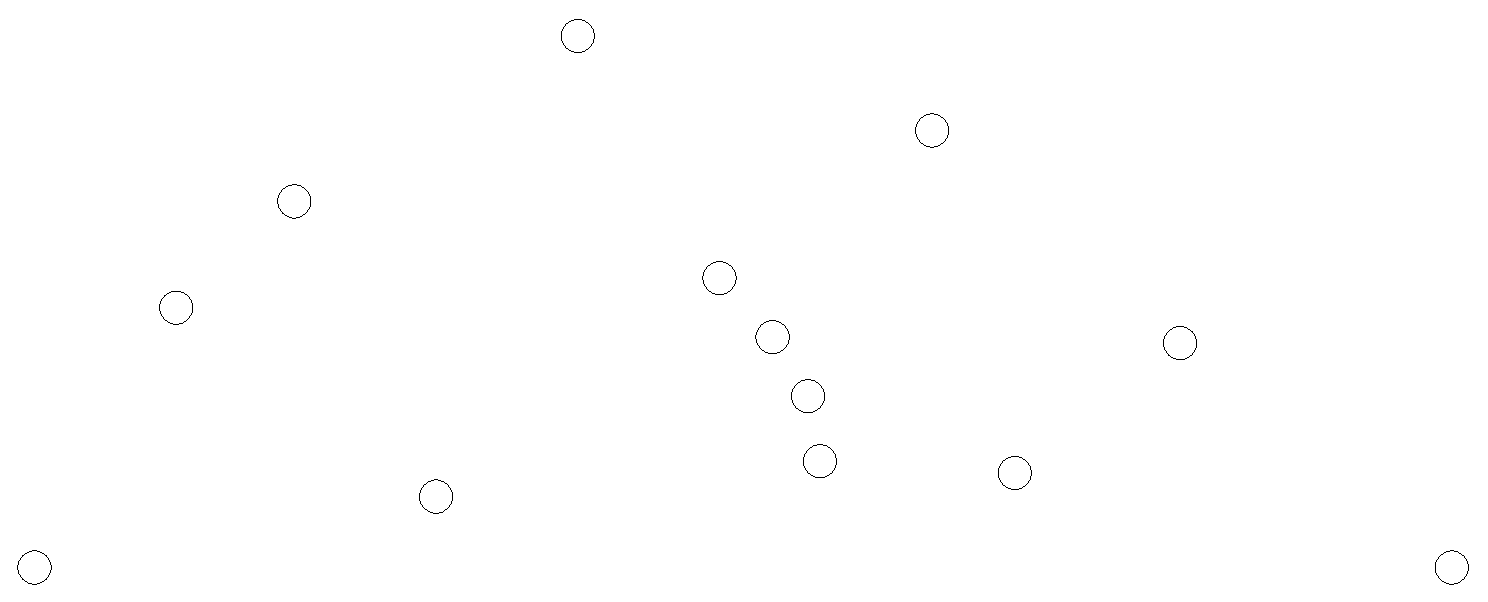
\includegraphics[width=\textwidth]{points}
  \begin{example}
    For the convex hull, a list of triangles and the points they
    cover.
  \end{example}
\end{frame}


\section{Open Problems}




\begin{frame}
\frametitle{Open Problems}
\begin{itemize}
% \subsection{Deferred Data Structures}
\item Deferred Data Structures 
  \begin{itemize}
\item Input Order Adaptivity for \textsc{Sorting}\hfill [Carlos Ochoa]
\item Synergistic Algorithms  for \textsc{Sorting}\hfill [Carlos Ochoa]
\item Synergistic Algorithms  for \textsc{2D Maxima}\hfill [Carlos Ochoa]
\item Other... \hfill [\alert{Open}]
  \end{itemize}

\vfill
% \subsection{Computational Geometry in High Dimension}
\item Computational Geometry
  \begin{itemize}
\item \textsc{Maxima}\hfill [Javiel Rojas]
\item \textsc{Klee}\hfill [Javiel Rojas]
\item \textsc{MaxDepth}\hfill [Javiel Rojas]
\item Other... \hfill [\alert{Open}]
  \end{itemize}
\vfill
% \subsection{Compression}
\item Compression
  \begin{itemize}
\item \textsc{Prefix Free Codes} (aka Huffman)\hfill [David Mu{\~n}oz]
\item \textsc{Minimax Trees} \hfill [\alert{Open}]
\item \textsc{Alphabetic Binary Search Trees} \hfill [\alert{Open}] \\ (aka Hu Tucker)
  \end{itemize}
  \end{itemize}
\end{frame}

\begin{frame}
\frametitle{Open Problems}
\begin{itemize}

% \subsection{Stringology}
\item Stringology
  \begin{itemize}
\item \textsc{Insert-Swap Edit Distance}\hfill {\tiny \cite{2015-SPIRE-AdaptiveComputationOfTheSwapInsertCorrectionDistance-BarbayPerez}}
\item \textsc{General Edit Distance}\hfill [\alert{Open}]
\item \textsc{Block Edit Distance}\hfill [\alert{Open}]
  \end{itemize}
\vfill
% \subsection{Planar Graphs}
\item Planar Graphs
  \begin{itemize}
\item \textsc{Directed Max $(s,t)$ Flow} \hfill [\alert{Open}]
\item \textsc{Undirected Min $(s,t)$ Cut} \hfill [\alert{Open}]
  \end{itemize}
\item Searching
  \begin{itemize}
\item \textsc{Dynamic Search} Optimality \hfill [\alert{Open}]
  \end{itemize}
\item Set Combinations
  \begin{itemize}
\item \textsc{Conjunctive Queries} \hfill [\alert{Open}]
  \end{itemize}
\item Pattern Matching In Labelled Trees
  \begin{itemize}
\item \textsc{Path Subset Queries}  \hfill [\alert{Open}]
  \end{itemize}
\end{itemize}
\end{frame}


\section*{Summary}
\begin{frame}
  \frametitle<presentation>{Summary}

  \begin{itemize}
  \item Refining the standard worst case analysis (``\alert{BIG DATA''}).  
  \item The techniques can be applied to your favorite problem.
  \item Next semester: \alert{CC5109-Analisis Fino de Algoritmos y Estructuras de Datos}.
  \end{itemize}
  
  % The following outlook is optional.
  \vskip0pt plus.5fill
  \begin{itemize}
  \item
    Outlook
    \begin{itemize}
    \item This works also for Compressed Data Structures!
    \item The ultimate challenge is to obtain \emph{instance optimal} results, 
    \item in particular  \alert{$1$-instance optimality}!
    \end{itemize}
  \end{itemize}
\end{frame}

\begin{frame}
\frametitle{For Potential Students}
\begin{itemize}
\item Funds
  \begin{itemize}
\item Fondecyt (Computational Geometry)
\item Nucleo (Theory)
  \end{itemize}
\item International Contacts
\end{itemize}
\end{frame}


\begin{frame}
  \frametitle<presentation>{Bibliography}
\nocite{2013-IanFest-FromTimeToSpace-Barbay}
\nocite{2009-FOCS-InstanceOptimalGeometricAlgorithms-AfshaniBarbayChan}
\nocite{2013-CCCG-MaximumWeightPlanarBoxesInON2TimeAndBetter-BarbayChanNavarroPerezLantero}

\tiny

\bibliographystyle{apalike}

\bibliography{/home/jbarbay/EverGoing/Bibliography/bibliographyDatabaseJeremyBarbay,/home/jbarbay/EverGoing/Publications/publications-ExportedFromOrgmode-Barbay}

\end{frame}


\appendix

\section{More details}
\subsection{Prefix Free Codes and variants}

\begin{frame}
  \frametitle{Optimal Prefix Free Codes [In Progress]}
  \begin{itemize}
  \item $O(n\lg n)$ classical algorithm.
  \begin{itemize}
  \item $O(n)$ algorithm when frequencies are sorted.
  \item $O(n)$ algorithm when frequencies are all within a factor of $2$.
  \item $O(n)$ algorithm when frequencies are all distinct by factor of $2$.
    \end{itemize}
  \item Adaptive Results for $k$ distinct code lengths:
    \begin{itemize}
     \item Belal and Elmasry claim $O(nk)$ in STACS 2006. 
     \item Belal and Elmasry claim $O(n 4^k)$ in ARXIV 2012.
  \item A lower bound of \alert{$\Omega(n\lg k)$} in the worst case over
  instances resulting in $k$ distinct code lengths.
     \end{itemize}
\item Conjectures:
  \begin{itemize}
  \item $O(n\lg k)$ adaptive algorithm?
  \item $O(nH(n_1,\ldots,n_k))$ instance optimal algorithm?
  \item \alert{$O(n)$ algorithm in word-RAM} (vs $O(n\lg\lg n)$ for int. sorting)?
  \end{itemize}
  \end{itemize}
\end{frame}

\begin{frame}
  \frametitle{Optimal Minimax Trees [Open]}
  \begin{itemize}
\item Classical:
  \begin{itemize}
  \item Tree minimizing the max weight+height of a leaf.
  \item $O(n\lg n)$ classical algorithm [Golumbic];
    \end{itemize}
  \item Fine Grained Analysis Results:
  \begin{itemize}
  \item $O(n)$ algorithm when weights partially sorted by fractional part [Drmota, Szpankowski];
  \item $O(nd\lg\lg n)$ where $d$ is the number of distinct values
    $\lceil w_i\rceil$ [Kirkpatrick and Klawe]
  \item $O(n)$ algorithm in word-RAM [Gawrichowski,Gagie]!
    \end{itemize}
    \end{itemize}
\end{frame}

\begin{frame}
  \frametitle{Optimal Alphabetic Binary Search Tree [Open]}
  \begin{itemize}
  \item $O(n\lg n)$ classical \alert{Hu-Tucker} algorithm;
  \item Easy Cases:
  \begin{itemize}
  \item $o(n\lg n)$ algorithms in many particular cases;
  \item $O(n)$ algorithm when frequencies ``can be sorted in linear time'';
  \item A lower bound of $\Omega(n\lg k)$ in the worst case over
    instances resulting in $k$ distinct code lengths.
    \end{itemize}
  \item Conjectures:
  \begin{itemize}
  \item $O(n\lg k)$ adaptive algorithm?
  \item $O(nH(n_1,\ldots,n_k))$ instance optimal algorithm?
  \item \alert{$O(n)$ algorithm in word-RAM}?
  \end{itemize}

    \end{itemize}
\end{frame}

\subsection{Planar Graph Algorithms}
  \begin{frame}
    \frametitle{Directed Max $(s,t)$ Flow [Open]}
\vspace{3cm}
    \begin{itemize}
    \item $O(n\lg n)$ classical algorithm;
    \item $O(n)$ well known algorithm when $s$ and $t$ share a face;
    \item $O(nk)$ new algorithm, where $k$ is the number of edges
      between $s$ and $t$;
    \end{itemize}
  \end{frame}

  \begin{frame}
    \frametitle{Undirected Min $(s,t)$ Cut [Open]}
\vspace{3cm}
    \begin{itemize}
    \item $O(n\lg n)$ well known algorithm
    \item $O(n\lg k)$ recent algorithm (STACS 2011!)
    \item Can this be improved?
    \end{itemize}
  \end{frame}

  \begin{INUTILE}
  \subsection{Others Fields?}

  \begin{frame}
  \frametitle{Other Fields}
  \begin{itemize}
\item Edit Distance
  \begin{itemize}
\item Swap Insert \cite{2015-SPIRE-AdaptiveComputationOfTheSwapInsertCorrectionDistance-BarbayPerez}
\item Others
  \end{itemize}
\item Pattern Matching
\item
  \end{itemize}
  \end{frame}
  \end{INUTILE}



%%% Local Variables:
%%% mode: latex
%%% TeX-master: "2016-Santiago-FromFineGrainedAnalysisToInstanceOptimality-Barbay"
%%% End:


\end{document}



%%% Local Variables:
%%% mode: latex
%%% TeX-master: t
%%% End:
